% Options for packages loaded elsewhere
\PassOptionsToPackage{unicode}{hyperref}
\PassOptionsToPackage{hyphens}{url}
%
\documentclass[
]{article}
\usepackage{lmodern}
\usepackage{amssymb,amsmath}
\usepackage{ifxetex,ifluatex}
\ifnum 0\ifxetex 1\fi\ifluatex 1\fi=0 % if pdftex
  \usepackage[T1]{fontenc}
  \usepackage[utf8]{inputenc}
  \usepackage{textcomp} % provide euro and other symbols
\else % if luatex or xetex
  \usepackage{unicode-math}
  \defaultfontfeatures{Scale=MatchLowercase}
  \defaultfontfeatures[\rmfamily]{Ligatures=TeX,Scale=1}
\fi
% Use upquote if available, for straight quotes in verbatim environments
\IfFileExists{upquote.sty}{\usepackage{upquote}}{}
\IfFileExists{microtype.sty}{% use microtype if available
  \usepackage[]{microtype}
  \UseMicrotypeSet[protrusion]{basicmath} % disable protrusion for tt fonts
}{}
\makeatletter
\@ifundefined{KOMAClassName}{% if non-KOMA class
  \IfFileExists{parskip.sty}{%
    \usepackage{parskip}
  }{% else
    \setlength{\parindent}{0pt}
    \setlength{\parskip}{6pt plus 2pt minus 1pt}}
}{% if KOMA class
  \KOMAoptions{parskip=half}}
\makeatother
\usepackage{xcolor}
\IfFileExists{xurl.sty}{\usepackage{xurl}}{} % add URL line breaks if available
\IfFileExists{bookmark.sty}{\usepackage{bookmark}}{\usepackage{hyperref}}
\hypersetup{
  pdftitle={Setting up a zooplankton model using mizer},
  pdfauthor={Patrick Sykes},
  hidelinks,
  pdfcreator={LaTeX via pandoc}}
\urlstyle{same} % disable monospaced font for URLs
\usepackage[margin=1in]{geometry}
\usepackage{color}
\usepackage{fancyvrb}
\newcommand{\VerbBar}{|}
\newcommand{\VERB}{\Verb[commandchars=\\\{\}]}
\DefineVerbatimEnvironment{Highlighting}{Verbatim}{commandchars=\\\{\}}
% Add ',fontsize=\small' for more characters per line
\usepackage{framed}
\definecolor{shadecolor}{RGB}{248,248,248}
\newenvironment{Shaded}{\begin{snugshade}}{\end{snugshade}}
\newcommand{\AlertTok}[1]{\textcolor[rgb]{0.94,0.16,0.16}{#1}}
\newcommand{\AnnotationTok}[1]{\textcolor[rgb]{0.56,0.35,0.01}{\textbf{\textit{#1}}}}
\newcommand{\AttributeTok}[1]{\textcolor[rgb]{0.77,0.63,0.00}{#1}}
\newcommand{\BaseNTok}[1]{\textcolor[rgb]{0.00,0.00,0.81}{#1}}
\newcommand{\BuiltInTok}[1]{#1}
\newcommand{\CharTok}[1]{\textcolor[rgb]{0.31,0.60,0.02}{#1}}
\newcommand{\CommentTok}[1]{\textcolor[rgb]{0.56,0.35,0.01}{\textit{#1}}}
\newcommand{\CommentVarTok}[1]{\textcolor[rgb]{0.56,0.35,0.01}{\textbf{\textit{#1}}}}
\newcommand{\ConstantTok}[1]{\textcolor[rgb]{0.00,0.00,0.00}{#1}}
\newcommand{\ControlFlowTok}[1]{\textcolor[rgb]{0.13,0.29,0.53}{\textbf{#1}}}
\newcommand{\DataTypeTok}[1]{\textcolor[rgb]{0.13,0.29,0.53}{#1}}
\newcommand{\DecValTok}[1]{\textcolor[rgb]{0.00,0.00,0.81}{#1}}
\newcommand{\DocumentationTok}[1]{\textcolor[rgb]{0.56,0.35,0.01}{\textbf{\textit{#1}}}}
\newcommand{\ErrorTok}[1]{\textcolor[rgb]{0.64,0.00,0.00}{\textbf{#1}}}
\newcommand{\ExtensionTok}[1]{#1}
\newcommand{\FloatTok}[1]{\textcolor[rgb]{0.00,0.00,0.81}{#1}}
\newcommand{\FunctionTok}[1]{\textcolor[rgb]{0.00,0.00,0.00}{#1}}
\newcommand{\ImportTok}[1]{#1}
\newcommand{\InformationTok}[1]{\textcolor[rgb]{0.56,0.35,0.01}{\textbf{\textit{#1}}}}
\newcommand{\KeywordTok}[1]{\textcolor[rgb]{0.13,0.29,0.53}{\textbf{#1}}}
\newcommand{\NormalTok}[1]{#1}
\newcommand{\OperatorTok}[1]{\textcolor[rgb]{0.81,0.36,0.00}{\textbf{#1}}}
\newcommand{\OtherTok}[1]{\textcolor[rgb]{0.56,0.35,0.01}{#1}}
\newcommand{\PreprocessorTok}[1]{\textcolor[rgb]{0.56,0.35,0.01}{\textit{#1}}}
\newcommand{\RegionMarkerTok}[1]{#1}
\newcommand{\SpecialCharTok}[1]{\textcolor[rgb]{0.00,0.00,0.00}{#1}}
\newcommand{\SpecialStringTok}[1]{\textcolor[rgb]{0.31,0.60,0.02}{#1}}
\newcommand{\StringTok}[1]{\textcolor[rgb]{0.31,0.60,0.02}{#1}}
\newcommand{\VariableTok}[1]{\textcolor[rgb]{0.00,0.00,0.00}{#1}}
\newcommand{\VerbatimStringTok}[1]{\textcolor[rgb]{0.31,0.60,0.02}{#1}}
\newcommand{\WarningTok}[1]{\textcolor[rgb]{0.56,0.35,0.01}{\textbf{\textit{#1}}}}
\usepackage{graphicx,grffile}
\makeatletter
\def\maxwidth{\ifdim\Gin@nat@width>\linewidth\linewidth\else\Gin@nat@width\fi}
\def\maxheight{\ifdim\Gin@nat@height>\textheight\textheight\else\Gin@nat@height\fi}
\makeatother
% Scale images if necessary, so that they will not overflow the page
% margins by default, and it is still possible to overwrite the defaults
% using explicit options in \includegraphics[width, height, ...]{}
\setkeys{Gin}{width=\maxwidth,height=\maxheight,keepaspectratio}
% Set default figure placement to htbp
\makeatletter
\def\fps@figure{htbp}
\makeatother
\setlength{\emergencystretch}{3em} % prevent overfull lines
\providecommand{\tightlist}{%
  \setlength{\itemsep}{0pt}\setlength{\parskip}{0pt}}
\setcounter{secnumdepth}{-\maxdimen} % remove section numbering

\title{Setting up a zooplankton model using mizer}
\author{Patrick Sykes}
\date{2021-03-09}

\begin{document}
\maketitle

\hypertarget{introduction}{%
\section{Introduction}\label{introduction}}

Here we will recreate the ZooMSS model (version 2) in Heneghan et
al.~(2020) using mizer.

There are some benefits to doing this. The main things for us are that
mizer has a lot of functionality already that we would like to bring to
ZooMSS, and a growing community that we can learn from and contribute
to.

There are a few important differences between the models (as I found out
along the way). The most fundamental of these is that the governing PDE
is in a different form in each model (ZooMSS works in absolute abundance
over log-weight size classes, and mizer uses normalised abundance and
absolute-weight size classes), and hence the numerics work out a bit
differently. As we will see, ``recreating'' ZooMSS in mizer required
changing the numerics in mizer to match how they work out in ZooMSS.

Let's get started! We begin with some setup of required packages.

\begin{Shaded}
\begin{Highlighting}[]
\CommentTok{#get required packages}
\KeywordTok{library}\NormalTok{(devtools)}
\CommentTok{#most up to date master branch of mizer}
\CommentTok{#install_github("sizespectrum/mizer")}
\CommentTok{#install_github("astaaudzi/mizer-rewiring", ref = "temp-model-comp")}
\CommentTok{#documentation here:}
\CommentTok{#https://sizespectrum.org/mizer/dev/index.html}
\KeywordTok{library}\NormalTok{(mizer)}
\KeywordTok{require}\NormalTok{(tidyverse)}

\CommentTok{#remotes::install_github("sizespectrum/mizerExperimental")}
\KeywordTok{library}\NormalTok{(mizerExperimental)}

\CommentTok{#library(plotly)}
\end{Highlighting}
\end{Shaded}

\hypertarget{set-up-mizer-model}{%
\subsection{Set-up mizer model}\label{set-up-mizer-model}}

Next let's read in the parameters from ZooMSS.

\begin{Shaded}
\begin{Highlighting}[]
\NormalTok{groups <-}\KeywordTok{read_csv}\NormalTok{(}\StringTok{"data/TestGroups_mizer.csv"}\NormalTok{)}
\end{Highlighting}
\end{Shaded}

\begin{verbatim}
## Parsed with column specification:
## cols(
##   species = col_character(),
##   Type = col_character(),
##   FeedType = col_character(),
##   Prop = col_double(),
##   w_min = col_double(),
##   w_inf = col_double(),
##   w_mat = col_double(),
##   gamma = col_double(),
##   q = col_double(),
##   PPMRscale = col_double(),
##   PPMR = col_double(),
##   FeedWidth = col_double(),
##   GrossGEscale = col_double(),
##   Carbon = col_double(),
##   Repro = col_double(),
##   PlotColour = col_character(),
##   interaction_resource = col_double()
## )
\end{verbatim}

\begin{Shaded}
\begin{Highlighting}[]
\NormalTok{groups}\OperatorTok{$}\NormalTok{w_min <-}\StringTok{ }\DecValTok{10}\OperatorTok{^}\NormalTok{groups}\OperatorTok{$}\NormalTok{w_min }\CommentTok{#convert from log10 values}
\NormalTok{groups}\OperatorTok{$}\NormalTok{w_inf <-}\StringTok{ }\DecValTok{10}\OperatorTok{^}\NormalTok{groups}\OperatorTok{$}\NormalTok{w_inf}
\NormalTok{groups}\OperatorTok{$}\NormalTok{w_mat <-}\StringTok{ }\DecValTok{10}\OperatorTok{^}\NormalTok{groups}\OperatorTok{$}\NormalTok{w_mat}
\NormalTok{groups}\OperatorTok{$}\NormalTok{h <-}\StringTok{ }\FloatTok{1e50} \CommentTok{# should be Inf, but that breaks the calculations. Massive value still works out to effectively unlimited feeding as allowed in ZooMSS - not currently being used anyway.}
\NormalTok{groups}\OperatorTok{$}\NormalTok{ks <-}\StringTok{ }\DecValTok{0} \CommentTok{#turn off standard metabolism}
\CommentTok{#todo - ramp up constant repro for coexistence}

\CommentTok{# read interaction matrix}
\CommentTok{# get the interaction matrix - actually I think we can leave this out. Default is all 1s, which is the same as in ZooMSS. Included for completeness; it may be useful in future to keep this in.}
\NormalTok{theta <-}\StringTok{ }\KeywordTok{readRDS}\NormalTok{(}\StringTok{"data/zoomss_inter.rds"}\NormalTok{)[,}\OperatorTok{-}\DecValTok{1}\NormalTok{]}
\end{Highlighting}
\end{Shaded}

We will pass these parameters to mizer to set up a new multispecies
model.

\begin{Shaded}
\begin{Highlighting}[]
\NormalTok{ID <-}\StringTok{ }\DecValTok{223} \CommentTok{#index of environmental data to choose}
\NormalTok{envirofull <-}\StringTok{ }\KeywordTok{readRDS}\NormalTok{(}\StringTok{"data/envirofull_20200317.RDS"}\NormalTok{)}
\NormalTok{enviro_row <-}\StringTok{ }\NormalTok{envirofull[envirofull}\OperatorTok{$}\NormalTok{cellID}\OperatorTok{==}\NormalTok{ID,]}

\CommentTok{#set up the fixed phyoplankton spectrum}
\NormalTok{phyto_fixed <-}\StringTok{ }\ControlFlowTok{function}\NormalTok{(params, n, n_pp, n_other, rates, dt, }\DataTypeTok{kappa=}\NormalTok{params}\OperatorTok{@}\NormalTok{resource_params}\OperatorTok{$}\NormalTok{kappa, }\DataTypeTok{lambda=}\NormalTok{params}\OperatorTok{@}\NormalTok{resource_params}\OperatorTok{$}\NormalTok{lambda, ... ) \{}
\NormalTok{  npp <-}\StringTok{ }\NormalTok{kappa}\OperatorTok{*}\NormalTok{params}\OperatorTok{@}\NormalTok{w_full}\OperatorTok{^}\NormalTok{(}\DecValTok{1}\OperatorTok{-}\NormalTok{lambda) }\OperatorTok{/}\StringTok{ }\NormalTok{params}\OperatorTok{@}\NormalTok{dw_full }\CommentTok{#returns the fixed spectrum at every time step}
\NormalTok{  npp[params}\OperatorTok{@}\NormalTok{w_full }\OperatorTok{>}\StringTok{ }\NormalTok{params}\OperatorTok{@}\NormalTok{resource_params}\OperatorTok{$}\NormalTok{w_pp_cutoff}\OperatorTok{*}\StringTok{ }\NormalTok{(}\DecValTok{1} \OperatorTok{-}\StringTok{ }\FloatTok{1e-06}\NormalTok{)] <-}\StringTok{ }\DecValTok{0}
  \KeywordTok{return}\NormalTok{(npp)}
\NormalTok{\}}

\NormalTok{mf.params <-}\StringTok{ }\KeywordTok{newMultispeciesParams}\NormalTok{(}\DataTypeTok{species_params=}\NormalTok{groups,}
                                   \DataTypeTok{interaction=}\OtherTok{NULL}\NormalTok{, }\CommentTok{#NULL sets all to 1, no strict herbivores}
                                   \DataTypeTok{no_w =} \DecValTok{178}\NormalTok{, }\CommentTok{#number of zoo+fish size classes;}
                                   \DataTypeTok{min_w_pp =} \DecValTok{10}\OperatorTok{^}\NormalTok{(}\OperatorTok{-}\FloatTok{14.4}\NormalTok{), }\CommentTok{#minimum phyto size. Note: use -14.4, not -14.5, otherwise it makes an extra size class}
                                   \DataTypeTok{w_pp_cutoff =} \DecValTok{10}\OperatorTok{^}\NormalTok{(enviro_row}\OperatorTok{$}\NormalTok{phyto_max), }\CommentTok{#maximum phyto size}
                                   \DataTypeTok{n =} \FloatTok{0.7}\NormalTok{, }\CommentTok{#The allometric growth exponent used in ZooMSS}
                                   \DataTypeTok{z0pre =} \DecValTok{1}\NormalTok{, }\CommentTok{#external mortality (senescence)}
                                   \DataTypeTok{z0exp =} \FloatTok{0.3}\NormalTok{,}
                                   \DataTypeTok{resource_dynamics =} \StringTok{"phyto_fixed"}\NormalTok{,}
                                   \DataTypeTok{kappa =} \DecValTok{10}\OperatorTok{^}\NormalTok{(enviro_row}\OperatorTok{$}\NormalTok{phyto_int), }
                                   \DataTypeTok{lambda =} \DecValTok{1}\OperatorTok{-}\NormalTok{enviro_row}\OperatorTok{$}\NormalTok{phyto_slope,}
                                   \CommentTok{#RDD = constantRDD(species_params = groups) #first go at this}
                                   \CommentTok{#pred_kernel = ... #probably easiest to just import this/pre-calculate it, once dimensions are worked out}
\NormalTok{)}
\end{Highlighting}
\end{Shaded}

\begin{verbatim}
## Note: Using z0 = z0pre * w_inf ^ z0exp for missing z0 values.
\end{verbatim}

\begin{Shaded}
\begin{Highlighting}[]
\CommentTok{#checks that there are as many phytoplankton size classes as ZooMSS}
\KeywordTok{length}\NormalTok{(}\KeywordTok{which}\NormalTok{(mf.params}\OperatorTok{@}\NormalTok{initial_n_pp}\OperatorTok{>}\DecValTok{0}\NormalTok{)) }\OperatorTok{==}\StringTok{ }\KeywordTok{length}\NormalTok{(}\KeywordTok{seq}\NormalTok{(}\OperatorTok{-}\FloatTok{14.5}\NormalTok{,enviro_row}\OperatorTok{$}\NormalTok{phyto_max, }\DataTypeTok{by =} \FloatTok{0.1}\NormalTok{))}
\end{Highlighting}
\end{Shaded}

\begin{verbatim}
## [1] TRUE
\end{verbatim}

Now do some fiddling to make the new MizerParams object match the ZooMSS
parameters. Note: this chunk is adapted from \texttt{fZooMSS\_setup.R},
found at \url{https://github.com/MathMarEcol/ZooMSS/}.

\begin{Shaded}
\begin{Highlighting}[]
\NormalTok{mf.params}\OperatorTok{@}\NormalTok{other_params}\OperatorTok{$}\NormalTok{temp_eff <-}\StringTok{  }\KeywordTok{matrix}\NormalTok{(}\FloatTok{2.}\OperatorTok{^}\NormalTok{((enviro_row}\OperatorTok{$}\NormalTok{sst }\OperatorTok{-}\StringTok{ }\DecValTok{30}\NormalTok{)}\OperatorTok{/}\DecValTok{10}\NormalTok{), }\DataTypeTok{nrow =} \KeywordTok{length}\NormalTok{(mf.params}\OperatorTok{@}\NormalTok{species_params}\OperatorTok{$}\NormalTok{species), }\DataTypeTok{ncol =} \KeywordTok{length}\NormalTok{(mf.params}\OperatorTok{@}\NormalTok{w))}

\NormalTok{setZooMizerConstants <-}\StringTok{ }\ControlFlowTok{function}\NormalTok{(params, Groups, sst)\{}
  \CommentTok{#### CALCULATES CONSTANT BITS OF THE MODEL FUNCTIONS FOR EACH GROUP}
\NormalTok{  SearchVol <-}\StringTok{ }\KeywordTok{getSearchVolume}\NormalTok{(params)}
\NormalTok{  M_sb <-}\StringTok{ }\KeywordTok{getExtMort}\NormalTok{(params)}
\NormalTok{  ZSpre <-}\StringTok{ }\DecValTok{1} \CommentTok{# senescence mortality prefactor}
\NormalTok{  ZSexp <-}\StringTok{ }\FloatTok{0.3} \CommentTok{# senescence mortality exponent}

\NormalTok{  pred_kernel <-}\StringTok{ }\KeywordTok{getPredKernel}\NormalTok{(params)}
\NormalTok{  prey_weight_matrix <-}\StringTok{ }\KeywordTok{matrix}\NormalTok{(params}\OperatorTok{@}\NormalTok{w_full, }\DataTypeTok{nrow =} \KeywordTok{length}\NormalTok{(params}\OperatorTok{@}\NormalTok{w), }\DataTypeTok{ncol =} \KeywordTok{length}\NormalTok{(params}\OperatorTok{@}\NormalTok{w_full), }\DataTypeTok{byrow =} \OtherTok{TRUE}\NormalTok{)}
\NormalTok{  pred_weight_matrix <-}\StringTok{ }\KeywordTok{matrix}\NormalTok{(params}\OperatorTok{@}\NormalTok{w, }\DataTypeTok{nrow =} \KeywordTok{length}\NormalTok{(params}\OperatorTok{@}\NormalTok{w), }\DataTypeTok{ncol =} \KeywordTok{length}\NormalTok{(params}\OperatorTok{@}\NormalTok{w_full))}

  \ControlFlowTok{for}\NormalTok{ (i }\ControlFlowTok{in} \DecValTok{1}\OperatorTok{:}\KeywordTok{nrow}\NormalTok{(params}\OperatorTok{@}\NormalTok{species_params)) \{}
    \CommentTok{## Senescence mortality}
    \ControlFlowTok{if}\NormalTok{ (params}\OperatorTok{@}\NormalTok{species_params}\OperatorTok{$}\NormalTok{Type[i] }\OperatorTok{==}\StringTok{ "Zooplankton"}\NormalTok{) \{}
\NormalTok{      M_sb[i,] <-}\StringTok{ }\NormalTok{ZSpre}\OperatorTok{*}\NormalTok{(params}\OperatorTok{@}\NormalTok{w}\OperatorTok{/}\NormalTok{(params}\OperatorTok{@}\NormalTok{species_params}\OperatorTok{$}\NormalTok{w_mat[i]))}\OperatorTok{^}\NormalTok{ZSexp}
\NormalTok{      M_sb[i, params}\OperatorTok{@}\NormalTok{species_params}\OperatorTok{$}\NormalTok{w_inf[i] }\OperatorTok{<}\StringTok{ }\NormalTok{params}\OperatorTok{@}\NormalTok{w }\OperatorTok{*}\StringTok{ }\NormalTok{(}\DecValTok{1} \OperatorTok{+}\StringTok{ }\FloatTok{1e-06}\NormalTok{)] <-}\StringTok{ }\DecValTok{0}
\NormalTok{      M_sb[i, params}\OperatorTok{@}\NormalTok{species_params}\OperatorTok{$}\NormalTok{w_mat[i] }\OperatorTok{>}\StringTok{ }\NormalTok{params}\OperatorTok{@}\NormalTok{w }\OperatorTok{*}\StringTok{ }\NormalTok{(}\DecValTok{1} \OperatorTok{-}\StringTok{ }\FloatTok{1e-06}\NormalTok{)] <-}\StringTok{ }\DecValTok{0}
\NormalTok{    \}}

    \ControlFlowTok{if}\NormalTok{ (params}\OperatorTok{@}\NormalTok{species_params}\OperatorTok{$}\NormalTok{Type[i] }\OperatorTok{==}\StringTok{ "Fish"}\NormalTok{) \{}
\NormalTok{      M_sb[i,] <-}\StringTok{ }\FloatTok{0.1}\OperatorTok{*}\NormalTok{ZSpre}\OperatorTok{*}\NormalTok{(params}\OperatorTok{@}\NormalTok{w}\OperatorTok{/}\NormalTok{(params}\OperatorTok{@}\NormalTok{species_params}\OperatorTok{$}\NormalTok{w_mat[i]))}\OperatorTok{^}\NormalTok{ZSexp}
\NormalTok{      M_sb[i, params}\OperatorTok{@}\NormalTok{species_params}\OperatorTok{$}\NormalTok{w_inf[i] }\OperatorTok{<}\StringTok{ }\NormalTok{params}\OperatorTok{@}\NormalTok{w }\OperatorTok{*}\StringTok{ }\NormalTok{(}\DecValTok{1} \OperatorTok{+}\StringTok{ }\FloatTok{1e-06}\NormalTok{)] <-}\StringTok{ }\DecValTok{0}
\NormalTok{      M_sb[i, params}\OperatorTok{@}\NormalTok{species_params}\OperatorTok{$}\NormalTok{w_mat[i] }\OperatorTok{>}\StringTok{ }\NormalTok{params}\OperatorTok{@}\NormalTok{w }\OperatorTok{*}\StringTok{ }\NormalTok{(}\DecValTok{1} \OperatorTok{-}\StringTok{ }\FloatTok{1e-06}\NormalTok{)] <-}\StringTok{ }\DecValTok{0}
\NormalTok{    \}}

    \CommentTok{### Search volume}
\NormalTok{    SearchVol[i,] <-}\StringTok{ }\NormalTok{(params}\OperatorTok{@}\NormalTok{species_params}\OperatorTok{$}\NormalTok{gamma[i])}\OperatorTok{*}\NormalTok{(params}\OperatorTok{@}\NormalTok{w}\OperatorTok{^}\NormalTok{(params}\OperatorTok{@}\NormalTok{species_params}\OperatorTok{$}\NormalTok{q[i]))}
\NormalTok{    SearchVol[i, params}\OperatorTok{@}\NormalTok{species_params}\OperatorTok{$}\NormalTok{w_inf[i] }\OperatorTok{<}\StringTok{ }\NormalTok{params}\OperatorTok{@}\NormalTok{w }\OperatorTok{*}\StringTok{ }\NormalTok{(}\DecValTok{1} \OperatorTok{+}\StringTok{ }\FloatTok{1e-06}\NormalTok{)] <-}\StringTok{ }\DecValTok{0}
\NormalTok{    SearchVol[i, params}\OperatorTok{@}\NormalTok{species_params}\OperatorTok{$}\NormalTok{w_min[i] }\OperatorTok{>}\StringTok{ }\NormalTok{params}\OperatorTok{@}\NormalTok{w }\OperatorTok{*}\StringTok{ }\NormalTok{(}\DecValTok{1} \OperatorTok{+}\StringTok{ }\FloatTok{1e-06}\NormalTok{)] <-}\StringTok{ }\DecValTok{0}

    \CommentTok{### Predation Kernels}
    \ControlFlowTok{if}\NormalTok{ (}\KeywordTok{is.na}\NormalTok{(params}\OperatorTok{@}\NormalTok{species_params}\OperatorTok{$}\NormalTok{PPMRscale[i]) }\OperatorTok{==}\StringTok{ }\OtherTok{FALSE}\NormalTok{)\{ }\CommentTok{# If group has an m-value (zooplankton)}
      \CommentTok{# Calculate PPMR for zooplankton, which changes according to body-size (Wirtz, 2012)}
\NormalTok{      D.z <-}\StringTok{ }\DecValTok{2}\OperatorTok{*}\NormalTok{(}\DecValTok{3}\OperatorTok{*}\NormalTok{params}\OperatorTok{@}\NormalTok{w}\OperatorTok{*}\FloatTok{1e12}\OperatorTok{/}\NormalTok{(}\DecValTok{4}\OperatorTok{*}\NormalTok{pi))}\OperatorTok{^}\NormalTok{(}\DecValTok{1}\OperatorTok{/}\DecValTok{3}\NormalTok{) }\CommentTok{# convert body mass g to ESD (um)}
\NormalTok{      betas <-}\StringTok{ }\NormalTok{(}\KeywordTok{exp}\NormalTok{(}\FloatTok{0.02}\OperatorTok{*}\KeywordTok{log}\NormalTok{(D.z)}\OperatorTok{^}\DecValTok{2} \OperatorTok{-}\StringTok{ }\NormalTok{params}\OperatorTok{@}\NormalTok{species_params}\OperatorTok{$}\NormalTok{PPMRscale[i] }\OperatorTok{+}\StringTok{ }\FloatTok{1.832}\NormalTok{))}\OperatorTok{^}\DecValTok{3} \CommentTok{# Wirtz's equation}
\NormalTok{      beta_mat <-}\StringTok{ }\KeywordTok{matrix}\NormalTok{(betas, }\DataTypeTok{nrow =} \KeywordTok{length}\NormalTok{(params}\OperatorTok{@}\NormalTok{w), }\DataTypeTok{ncol =} \KeywordTok{length}\NormalTok{(params}\OperatorTok{@}\NormalTok{w_full))}

      \CommentTok{# Calculate feeding kernels}
\NormalTok{      pred_kernel[i, , ] <-}\StringTok{ }\KeywordTok{exp}\NormalTok{(}\OperatorTok{-}\FloatTok{0.5}\OperatorTok{*}\NormalTok{(}\KeywordTok{log}\NormalTok{((beta_mat}\OperatorTok{*}\NormalTok{prey_weight_matrix) }\OperatorTok{/}
\StringTok{                                            }\NormalTok{pred_weight_matrix)}\OperatorTok{/}\NormalTok{params}\OperatorTok{@}\NormalTok{species_params}\OperatorTok{$}\NormalTok{FeedWidth[i])}\OperatorTok{^}\DecValTok{2}\NormalTok{) }\OperatorTok{/}
\StringTok{        }\KeywordTok{sqrt}\NormalTok{(}\DecValTok{2}\OperatorTok{*}\NormalTok{pi}\OperatorTok{*}\NormalTok{params}\OperatorTok{@}\NormalTok{species_params}\OperatorTok{$}\NormalTok{FeedWidth[i]}\OperatorTok{^}\DecValTok{2}\NormalTok{)}
      \CommentTok{# The feeding kernel of filter feeders is not expected to change  with increasing size so we fix it here}

      \CommentTok{# if (param$fixed_filterPPMR == TRUE)\{}
      \ControlFlowTok{if}\NormalTok{ (i }\OperatorTok{==}\StringTok{ }\DecValTok{3}\NormalTok{) \{}
\NormalTok{        pred_kernel[i, , ] <-}\StringTok{ }\KeywordTok{matrix}\NormalTok{(pred_kernel[i,}\DecValTok{44}\NormalTok{,], }\DataTypeTok{nrow =} \KeywordTok{length}\NormalTok{(params}\OperatorTok{@}\NormalTok{w), }\DataTypeTok{ncol =} \KeywordTok{length}\NormalTok{(params}\OperatorTok{@}\NormalTok{w_full), }\DataTypeTok{byrow =} \OtherTok{TRUE}\NormalTok{)}
\NormalTok{      \}}
      \ControlFlowTok{if}\NormalTok{ (i }\OperatorTok{==}\StringTok{ }\DecValTok{8}\NormalTok{) \{}
\NormalTok{        pred_kernel[i, , ] <-}\StringTok{ }\KeywordTok{matrix}\NormalTok{(pred_kernel[i,}\DecValTok{61}\NormalTok{,], }\DataTypeTok{nrow =} \KeywordTok{length}\NormalTok{(params}\OperatorTok{@}\NormalTok{w), }\DataTypeTok{ncol =} \KeywordTok{length}\NormalTok{(params}\OperatorTok{@}\NormalTok{w_full), }\DataTypeTok{byrow =} \OtherTok{TRUE}\NormalTok{)}
\NormalTok{      \}}
      \CommentTok{# \}}

\NormalTok{    \} }\ControlFlowTok{else}\NormalTok{ \{ }\CommentTok{# If group does not have an m-value (fish)}
\NormalTok{      beta_mat <-}\StringTok{ }\KeywordTok{matrix}\NormalTok{(params}\OperatorTok{@}\NormalTok{species_params}\OperatorTok{$}\NormalTok{PPMR[i], }\DataTypeTok{nrow =} \KeywordTok{length}\NormalTok{(params}\OperatorTok{@}\NormalTok{w), }\DataTypeTok{ncol =} \KeywordTok{length}\NormalTok{(params}\OperatorTok{@}\NormalTok{w_full))}

      \CommentTok{# Calculate feeding kernels}
\NormalTok{      pred_kernel[i, , ] <-}\StringTok{ }\KeywordTok{exp}\NormalTok{(}\OperatorTok{-}\FloatTok{0.5}\OperatorTok{*}\NormalTok{(}\KeywordTok{log}\NormalTok{((beta_mat}\OperatorTok{*}\NormalTok{prey_weight_matrix) }\OperatorTok{/}
\StringTok{                                            }\NormalTok{pred_weight_matrix) }\OperatorTok{/}\StringTok{ }\NormalTok{params}\OperatorTok{@}\NormalTok{species_params}\OperatorTok{$}\NormalTok{FeedWidth[i])}\OperatorTok{^}\DecValTok{2}\NormalTok{) }\OperatorTok{/}
\StringTok{        }\KeywordTok{sqrt}\NormalTok{(}\DecValTok{2}\OperatorTok{*}\NormalTok{pi}\OperatorTok{*}\NormalTok{params}\OperatorTok{@}\NormalTok{species_params}\OperatorTok{$}\NormalTok{FeedWidth[i]}\OperatorTok{^}\DecValTok{2}\NormalTok{)}
\NormalTok{    \}}

\NormalTok{  \}}
\NormalTok{  SearchVol[}\DecValTok{12}\NormalTok{,}\DecValTok{178}\NormalTok{] <-}\StringTok{ }\NormalTok{(params}\OperatorTok{@}\NormalTok{species_params}\OperatorTok{$}\NormalTok{gamma[}\DecValTok{12}\NormalTok{])}\OperatorTok{*}\NormalTok{(params}\OperatorTok{@}\NormalTok{w[}\DecValTok{178}\NormalTok{]}\OperatorTok{^}\NormalTok{(params}\OperatorTok{@}\NormalTok{species_params}\OperatorTok{$}\NormalTok{q[}\DecValTok{12}\NormalTok{])) }\CommentTok{#adding last size class by hand}

  \CommentTok{#temperature effect}
\NormalTok{  M_sb <-}\StringTok{ }\NormalTok{params}\OperatorTok{@}\NormalTok{other_params}\OperatorTok{$}\NormalTok{temp_eff }\OperatorTok{*}\StringTok{ }\NormalTok{M_sb }\OperatorTok{*}\StringTok{ }\DecValTok{10} \CommentTok{# Incorporate temp effect on senscence mortality}


\NormalTok{  params}\OperatorTok{@}\NormalTok{initial_n_pp <-}\StringTok{ }\NormalTok{params}\OperatorTok{@}\NormalTok{resource_params}\OperatorTok{$}\NormalTok{kappa }\OperatorTok{*}\StringTok{ }\NormalTok{params}\OperatorTok{@}\NormalTok{w_full}\OperatorTok{^}\NormalTok{(}\DecValTok{1} \OperatorTok{-}\StringTok{ }\NormalTok{params}\OperatorTok{@}\NormalTok{resource_params}\OperatorTok{$}\NormalTok{lambda)}\OperatorTok{/}\NormalTok{params}\OperatorTok{@}\NormalTok{dw_full}
\NormalTok{  params}\OperatorTok{@}\NormalTok{initial_n_pp[params}\OperatorTok{@}\NormalTok{w_full }\OperatorTok{>}\StringTok{ }\NormalTok{params}\OperatorTok{@}\NormalTok{resource_params}\OperatorTok{$}\NormalTok{w_pp_cutoff] <-}\StringTok{ }\DecValTok{0}


\NormalTok{  a_dynam <-}\StringTok{ }\NormalTok{(params}\OperatorTok{@}\NormalTok{resource_params}\OperatorTok{$}\NormalTok{kappa)}\OperatorTok{*}\NormalTok{(params}\OperatorTok{@}\NormalTok{w[}\DecValTok{1}\NormalTok{]}\OperatorTok{^}\NormalTok{(}\DecValTok{2} \OperatorTok{-}\StringTok{ }\NormalTok{params}\OperatorTok{@}\NormalTok{resource_params}\OperatorTok{$}\NormalTok{lambda))}\CommentTok{#/params@dw[1] # calculate coefficient for initial dynamic spectrum, so that N(w_phyto) equals N(w_dynam) at w[1]}

  \CommentTok{# Initial abundances form a continuation of the plankton spectrum, with a slope of -1}
\NormalTok{  tempN <-}\StringTok{ }\KeywordTok{matrix}\NormalTok{(a_dynam}\OperatorTok{*}\NormalTok{(params}\OperatorTok{@}\NormalTok{w)}\OperatorTok{^}\NormalTok{(}\OperatorTok{-}\DecValTok{1}\NormalTok{)}\OperatorTok{/}\NormalTok{params}\OperatorTok{@}\NormalTok{dw, }\DataTypeTok{nrow =} \KeywordTok{nrow}\NormalTok{(params}\OperatorTok{@}\NormalTok{species_params), }\DataTypeTok{ncol =} \KeywordTok{length}\NormalTok{(params}\OperatorTok{@}\NormalTok{w), }\DataTypeTok{byrow =} \OtherTok{TRUE}\NormalTok{)}
\NormalTok{  props_z <-}\StringTok{ }\NormalTok{params}\OperatorTok{@}\NormalTok{species_params}\OperatorTok{$}\NormalTok{Prop[params}\OperatorTok{@}\NormalTok{species_params}\OperatorTok{$}\NormalTok{Type }\OperatorTok{==}\StringTok{ "Zooplankton"}\NormalTok{] }\CommentTok{# Zooplankton proportions}
\NormalTok{  tempN[params}\OperatorTok{@}\NormalTok{species_params}\OperatorTok{$}\NormalTok{Type }\OperatorTok{==}\StringTok{ "Zooplankton"}\NormalTok{,] <-}\StringTok{ }\NormalTok{props_z }\OperatorTok{*}\StringTok{ }\NormalTok{tempN[params}\OperatorTok{@}\NormalTok{species_params}\OperatorTok{$}\NormalTok{Type }\OperatorTok{==}\StringTok{ "Zooplankton"}\NormalTok{,] }\CommentTok{# Set abundances of diff zoo groups based on smallest size class proportions}
\NormalTok{  tempN[params}\OperatorTok{@}\NormalTok{species_params}\OperatorTok{$}\NormalTok{Type }\OperatorTok{==}\StringTok{ "Fish"}\NormalTok{,] <-}\StringTok{ }\NormalTok{(}\DecValTok{1}\OperatorTok{/}\KeywordTok{sum}\NormalTok{(params}\OperatorTok{@}\NormalTok{species_params}\OperatorTok{$}\NormalTok{Type }\OperatorTok{==}\StringTok{ "Fish"}\NormalTok{)) }\OperatorTok{*}\StringTok{ }\NormalTok{tempN[params}\OperatorTok{@}\NormalTok{species_params}\OperatorTok{$}\NormalTok{Type}\OperatorTok{==}\StringTok{"Fish"}\NormalTok{,] }\CommentTok{# Set abundandances of fish groups based on smallest size class proportions}

  \CommentTok{# For each group, set densities at w > Winf and w < Wmin to 0}
\NormalTok{  params}\OperatorTok{@}\NormalTok{species_params}\OperatorTok{$}\NormalTok{w_min <-}\StringTok{ }\NormalTok{params}\OperatorTok{@}\NormalTok{w[params}\OperatorTok{@}\NormalTok{w_min_idx]}
\NormalTok{  tempN[}\KeywordTok{unlist}\NormalTok{(}\KeywordTok{tapply}\NormalTok{(}\KeywordTok{round}\NormalTok{(}\KeywordTok{log10}\NormalTok{(params}\OperatorTok{@}\NormalTok{w), }\DataTypeTok{digits =} \DecValTok{2}\NormalTok{), }\DecValTok{1}\OperatorTok{:}\KeywordTok{length}\NormalTok{(params}\OperatorTok{@}\NormalTok{w), }\ControlFlowTok{function}\NormalTok{(wx,Winf) Winf }\OperatorTok{<}\StringTok{ }\NormalTok{wx, }\DataTypeTok{Winf =} \KeywordTok{log10}\NormalTok{(params}\OperatorTok{@}\NormalTok{species_params}\OperatorTok{$}\NormalTok{w_inf)))] <-}\StringTok{ }\DecValTok{0}
\NormalTok{  tempN[}\KeywordTok{unlist}\NormalTok{(}\KeywordTok{tapply}\NormalTok{(params}\OperatorTok{@}\NormalTok{w, }\DecValTok{1}\OperatorTok{:}\KeywordTok{length}\NormalTok{(params}\OperatorTok{@}\NormalTok{w), }\ControlFlowTok{function}\NormalTok{(wx,Wmin) Wmin }\OperatorTok{>}\StringTok{ }\NormalTok{wx, }\DataTypeTok{Wmin =}\NormalTok{ params}\OperatorTok{@}\NormalTok{species_params}\OperatorTok{$}\NormalTok{w_min))] <-}\StringTok{ }\DecValTok{0}
  \CommentTok{#dimnames(tempN) <- dimnames(params@initial_n)}
\NormalTok{  params}\OperatorTok{@}\NormalTok{initial_n[] <-}\StringTok{ }\NormalTok{tempN}
  
\NormalTok{  SearchVol <-}\StringTok{ }\KeywordTok{readRDS}\NormalTok{(}\StringTok{"data/SearchVol.rds"}\NormalTok{)}
  
\NormalTok{  params <-}\StringTok{ }\KeywordTok{setExtMort}\NormalTok{(params, }\DataTypeTok{z0 =}\NormalTok{ M_sb)}
\NormalTok{  params <-}\StringTok{ }\KeywordTok{setSearchVolume}\NormalTok{(params, }\DataTypeTok{search_vol =}\NormalTok{ SearchVol)}
\NormalTok{  params <-}\StringTok{ }\KeywordTok{setPredKernel}\NormalTok{(params, pred_kernel)}

  \KeywordTok{return}\NormalTok{(params)}
\NormalTok{\}}


\NormalTok{mf.params <-}\StringTok{ }\KeywordTok{setZooMizerConstants}\NormalTok{(}\DataTypeTok{params =}\NormalTok{ mf.params, }\DataTypeTok{Groups =}\NormalTok{ groups, }\DataTypeTok{sst=}\NormalTok{ enviro_row}\OperatorTok{$}\NormalTok{sst)}
\end{Highlighting}
\end{Shaded}

Try running it:

\begin{Shaded}
\begin{Highlighting}[]
\NormalTok{sim <-}\StringTok{ }\KeywordTok{project}\NormalTok{(mf.params)}
\KeywordTok{plot}\NormalTok{(sim) }\CommentTok{#note feeding level means satiation - 0 since there's no satiation in this model.}
\end{Highlighting}
\end{Shaded}

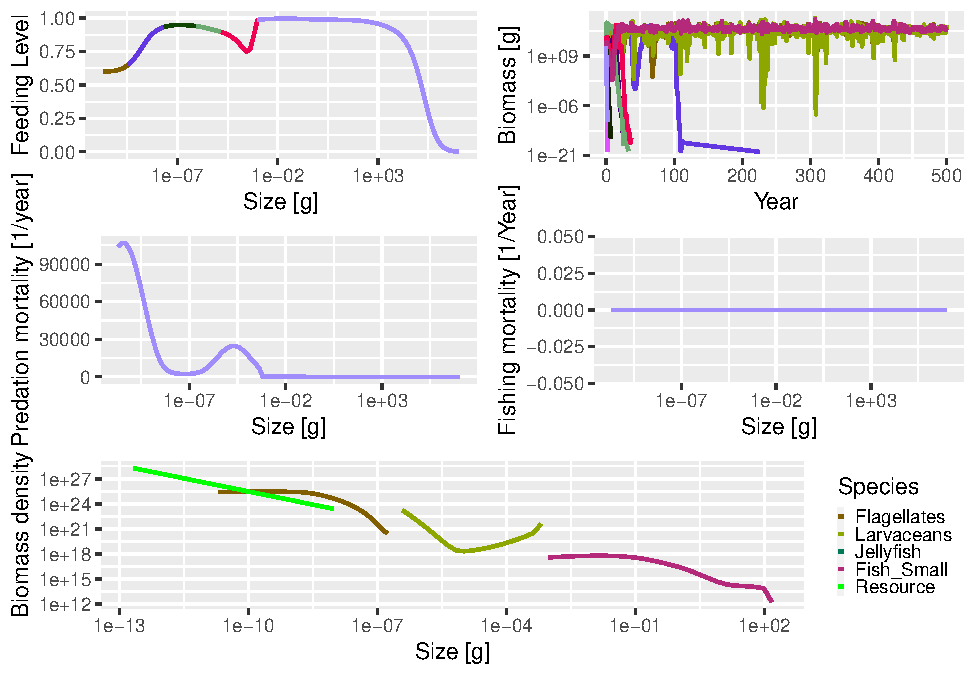
\includegraphics{setupModel_files/figure-latex/unnamed-chunk-4-1.pdf}

\begin{Shaded}
\begin{Highlighting}[]
\KeywordTok{plotBiomass}\NormalTok{(sim)}
\end{Highlighting}
\end{Shaded}

\includegraphics{setupModel_files/figure-latex/unnamed-chunk-4-2.pdf}

\begin{Shaded}
\begin{Highlighting}[]
\CommentTok{#plotlyGrowthCurves(sim,species="macrozooplankton")}
\CommentTok{#plotlyFeedingLevel(sim)}
\CommentTok{# feeding level satiation for some groups, except for the seabirds}
\CommentTok{# macrozooplankton - they are not growing enough,why?}
\CommentTok{#tuneParams(mf.params)}
\CommentTok{#plotlyGrowthCurves(sim,percentage = T)}
\KeywordTok{plotSpectra}\NormalTok{(sim, }\DataTypeTok{power =} \DecValTok{1}\NormalTok{)}
\end{Highlighting}
\end{Shaded}

\includegraphics{setupModel_files/figure-latex/unnamed-chunk-4-3.pdf}

Next thing to do is reproduction. In ZooMSS, this is handled by simply
setting the abundance in the smallest size class to be a fixed
proportion of the community size spectrum; in short

\[ N_i(w_{min}(i)) = prop(i) \sum_{j \neq i} N_j(w_{min}(i)),\] where
\(N_i(w)\) is the density of species \(i\) in weight class \(w\), and
\(prop(i)\) is a (fixed) proportion depending on the species.

In mizer, reproduction is linked to metabolism. The abundance in the
smallest size class is proportional to the energy available to mature
individuals for reproduction - i.e.~the energy left over after
subtracting metabolic costs (including energy to support growth) from
the energy assimilated (by mature individuals) from feeding on prey.

Now, to recreate this in mizer, we need to rewrite mizer's
\texttt{project\_simple()} function. We do this by making a new
function, \texttt{new\_project\_simple()}, and using it in place of the
default one. Note that there are two key changes in here: to change the
boundary conditions (``reproduction'') and to account for the conversion
from absolute abundance over logged weight classes in ZooMSS to
normalised abundance over absolute weight classes in ZooMizer (see the
PDF write-up of this - it was a bit of journey to first realise that
this could be a problem and then work out how to fix it).

\begin{Shaded}
\begin{Highlighting}[]
\NormalTok{new_project_simple <-}\StringTok{ }\ControlFlowTok{function}\NormalTok{(params, n, n_pp, n_other, t, dt, steps,}
\NormalTok{                               effort, resource_dynamics_fn, other_dynamics_fns,}
\NormalTok{                               rates_fns, ...) \{}
  \CommentTok{# Handy things}
\NormalTok{  no_sp <-}\StringTok{ }\KeywordTok{nrow}\NormalTok{(params}\OperatorTok{@}\NormalTok{species_params) }\CommentTok{# number of species}
\NormalTok{  no_w <-}\StringTok{ }\KeywordTok{length}\NormalTok{(params}\OperatorTok{@}\NormalTok{w) }\CommentTok{# number of fish size bins}
\NormalTok{  idx <-}\StringTok{ }\DecValTok{2}\OperatorTok{:}\NormalTok{no_w}
\NormalTok{  w_max_idx <-}\StringTok{ }\NormalTok{params}\OperatorTok{@}\NormalTok{w_min_idx}
  \ControlFlowTok{for}\NormalTok{ (i }\ControlFlowTok{in} \DecValTok{1}\OperatorTok{:}\KeywordTok{length}\NormalTok{(w_max_idx)) \{}
\NormalTok{    w_max_idx[i] <-}\StringTok{ }\KeywordTok{which}\NormalTok{(}\KeywordTok{round}\NormalTok{(}\KeywordTok{log10}\NormalTok{(params}\OperatorTok{@}\NormalTok{w),}\DecValTok{2}\NormalTok{) }\OperatorTok{==}\StringTok{ }\KeywordTok{round}\NormalTok{(}\KeywordTok{log10}\NormalTok{(params}\OperatorTok{@}\NormalTok{species_params}\OperatorTok{$}\NormalTok{w_inf[i]),}\DecValTok{2}\NormalTok{))}
\NormalTok{  \}}
  
\NormalTok{  fish_grps <-}\StringTok{ }\KeywordTok{which}\NormalTok{(params}\OperatorTok{@}\NormalTok{species_params}\OperatorTok{$}\NormalTok{Type }\OperatorTok{==}\StringTok{ "Fish"}\NormalTok{)}
  
  \ControlFlowTok{if}\NormalTok{(}\KeywordTok{sum}\NormalTok{(params}\OperatorTok{@}\NormalTok{species_params}\OperatorTok{$}\NormalTok{Type }\OperatorTok{==}\StringTok{ "Zooplankton"}\NormalTok{) }\OperatorTok{>}\StringTok{ }\DecValTok{1}\NormalTok{)\{ }\CommentTok{# If there's only one zoo group, then you do not need w0idx. All this stuff gives you info about all zoo groups except the smallest zoo group.}
\NormalTok{    w0idx <-}\StringTok{ }\KeywordTok{which}\NormalTok{(params}\OperatorTok{@}\NormalTok{w_min_idx }\OperatorTok{>}\StringTok{ }\KeywordTok{min}\NormalTok{(params}\OperatorTok{@}\NormalTok{w_min_idx) }\OperatorTok{&}\StringTok{ }\KeywordTok{is.na}\NormalTok{(params}\OperatorTok{@}\NormalTok{species_params}\OperatorTok{$}\NormalTok{Prop) }\OperatorTok{==}\StringTok{ }\OtherTok{FALSE}\NormalTok{)}
\NormalTok{    w0mins <-}\StringTok{ }\NormalTok{params}\OperatorTok{@}\NormalTok{w_min_idx[w0idx]}
\NormalTok{    props_z <-}\StringTok{ }\NormalTok{params}\OperatorTok{@}\NormalTok{species_params}\OperatorTok{$}\NormalTok{Prop[w0idx] }\CommentTok{# Zooplankton proportions}
\NormalTok{    \}}

  \CommentTok{# Hacky shortcut to access the correct element of a 2D array using 1D notation}
  \CommentTok{# This references the egg size bracket for all species, so for example}
  \CommentTok{# n[w_min_idx_array_ref] = n[,w_min_idx]}
\NormalTok{  w_min_idx_array_ref <-}\StringTok{ }\NormalTok{(params}\OperatorTok{@}\NormalTok{w_min_idx }\OperatorTok{-}\StringTok{ }\DecValTok{1}\NormalTok{) }\OperatorTok{*}\StringTok{ }\NormalTok{no_sp }\OperatorTok{+}\StringTok{ }\NormalTok{(}\DecValTok{1}\OperatorTok{:}\NormalTok{no_sp)}
  \CommentTok{# Matrices for solver}
\NormalTok{  a <-}\StringTok{ }\KeywordTok{matrix}\NormalTok{(}\DecValTok{0}\NormalTok{, }\DataTypeTok{nrow =}\NormalTok{ no_sp, }\DataTypeTok{ncol =}\NormalTok{ no_w)}
\NormalTok{  b <-}\StringTok{ }\KeywordTok{matrix}\NormalTok{(}\DecValTok{0}\NormalTok{, }\DataTypeTok{nrow =}\NormalTok{ no_sp, }\DataTypeTok{ncol =}\NormalTok{ no_w)}
\NormalTok{  S <-}\StringTok{ }\KeywordTok{matrix}\NormalTok{(}\DecValTok{0}\NormalTok{, }\DataTypeTok{nrow =}\NormalTok{ no_sp, }\DataTypeTok{ncol =}\NormalTok{ no_w)}

  \ControlFlowTok{for}\NormalTok{ (i_time }\ControlFlowTok{in} \DecValTok{1}\OperatorTok{:}\NormalTok{steps) \{}
\NormalTok{    r <-}\StringTok{ }\NormalTok{rates_fns}\OperatorTok{$}\KeywordTok{Rates}\NormalTok{(}
\NormalTok{      params, }\DataTypeTok{n =}\NormalTok{ n, }\DataTypeTok{n_pp =}\NormalTok{ n_pp, }\DataTypeTok{n_other =}\NormalTok{ n_other,}
      \DataTypeTok{t =}\NormalTok{ t, }\DataTypeTok{effort =}\NormalTok{ effort, }\DataTypeTok{rates_fns =}\NormalTok{ rates_fns, ...)}

    \CommentTok{# Update time}
\NormalTok{    t <-}\StringTok{ }\NormalTok{t }\OperatorTok{+}\StringTok{ }\NormalTok{dt}

    \CommentTok{# Update other components}
\NormalTok{    n_other_current <-}\StringTok{ }\NormalTok{n_other  }\CommentTok{# So that the resource dynamics can still}
    \CommentTok{# use the current value}
    \CommentTok{# for (component in names(params@other_dynamics)) \{}
    \CommentTok{#   n_other[[component]] <-}
    \CommentTok{#     other_dynamics_fns[[component]](}
    \CommentTok{#       params,}
    \CommentTok{#       n = n,}
    \CommentTok{#       n_pp = n_pp,}
    \CommentTok{#       n_other = n_other_current,}
    \CommentTok{#       rates = r,}
    \CommentTok{#       t = t,}
    \CommentTok{#       dt = dt,}
    \CommentTok{#       component = component,}
    \CommentTok{#       ...}
    \CommentTok{#     )}
    \CommentTok{# \}}

    \CommentTok{# Update resource}
    \CommentTok{# n_pp <- resource_dynamics_fn(params, n = n, n_pp = n_pp,}
    \CommentTok{#                              n_other = n_other_current, rates = r,}
    \CommentTok{#                              t = t, dt = dt, ...)}
\NormalTok{    n_pp <-}\StringTok{ }\NormalTok{n_pp}
    \CommentTok{# Iterate species one time step forward:}
    \CommentTok{# a_\{ij\} = - g_i(w_\{j-1\}) / dw_j dt}
\NormalTok{    a[, idx] <-}\StringTok{ }\KeywordTok{sweep}\NormalTok{(}\OperatorTok{-}\NormalTok{r}\OperatorTok{$}\NormalTok{e_growth[, idx }\OperatorTok{-}\StringTok{ }\DecValTok{1}\NormalTok{, }\DataTypeTok{drop =} \OtherTok{FALSE}\NormalTok{] }\OperatorTok{*}\StringTok{ }\NormalTok{dt, }\DecValTok{2}\NormalTok{,}
\NormalTok{                      params}\OperatorTok{@}\NormalTok{w[idx}\DecValTok{-1}\NormalTok{], }\StringTok{"/"}\NormalTok{) }\OperatorTok{*}\StringTok{ }\DecValTok{10}\OperatorTok{^}\NormalTok{(}\OperatorTok{-}\FloatTok{0.1}\NormalTok{) }\OperatorTok{/}\StringTok{ }\KeywordTok{log}\NormalTok{(}\DecValTok{10}\NormalTok{)}
    \CommentTok{# b_\{ij\} = 1 + g_i(w_j) / dw_j dt + \textbackslash{}mu_i(w_j) dt}
\NormalTok{    b[] <-}\StringTok{ }\DecValTok{1} \OperatorTok{+}\StringTok{ }\KeywordTok{sweep}\NormalTok{(r}\OperatorTok{$}\NormalTok{e_growth }\OperatorTok{*}\StringTok{ }\NormalTok{dt , }\DecValTok{2}\NormalTok{, params}\OperatorTok{@}\NormalTok{w, }\StringTok{"/"}\NormalTok{) }\OperatorTok{/}\KeywordTok{log}\NormalTok{(}\DecValTok{10}\NormalTok{) }\OperatorTok{+}\StringTok{ }\NormalTok{r}\OperatorTok{$}\NormalTok{mort }\OperatorTok{*}\StringTok{ }\NormalTok{dt }\OperatorTok{*}\StringTok{ }\FloatTok{0.1}
    \CommentTok{# S_\{ij\} <- N_i(w_j)}
\NormalTok{    S[,idx] <-}\StringTok{ }\NormalTok{n[, idx, drop =}\StringTok{ }\OtherTok{FALSE}\NormalTok{]}
    \CommentTok{# Update n}
    \CommentTok{# for (i in 1:no_sp) # number of species assumed small, so no need to}
    \CommentTok{#                      vectorize this loop over species}
    \CommentTok{#     for (j in (params@w_min_idx[i]+1):no_w)}
    \CommentTok{#         n[i,j] <- (S[i,j] - A[i,j]*n[i,j-1]) / B[i,j]}
    \CommentTok{# This is implemented via Rcpp}
\NormalTok{    n <-}\StringTok{ }\KeywordTok{inner_project_loop}\NormalTok{(}\DataTypeTok{no_sp =}\NormalTok{ no_sp, }\DataTypeTok{no_w =}\NormalTok{ no_w, }\DataTypeTok{n =}\NormalTok{ n,}
                            \DataTypeTok{A =}\NormalTok{ a, }\DataTypeTok{B =}\NormalTok{ b, }\DataTypeTok{S =}\NormalTok{ S,}
                            \DataTypeTok{w_min_idx =}\NormalTok{ params}\OperatorTok{@}\NormalTok{w_min_idx)}
  

  \CommentTok{# Update first and last size groups of n}
  \CommentTok{#TODO: Make this a little less hacky}
  \CommentTok{#n[1,1] <- params@species_params$Prop[1]*n_pp[length(params@w_full)-length(params@w)+1]}
  \ControlFlowTok{if}\NormalTok{(}\KeywordTok{sum}\NormalTok{(params}\OperatorTok{@}\NormalTok{species_params}\OperatorTok{$}\NormalTok{Type }\OperatorTok{==}\StringTok{ "Zooplankton"}\NormalTok{) }\OperatorTok{>}\StringTok{ }\DecValTok{1}\NormalTok{)\{ }\CommentTok{# If you only have one zoo group, it will be locked to phyto spectrum so you do not need to do this}
    \ControlFlowTok{for}\NormalTok{(i }\ControlFlowTok{in} \DecValTok{1}\OperatorTok{:}\KeywordTok{length}\NormalTok{(w0idx))\{}
\NormalTok{      w_min_curr <-}\StringTok{ }\NormalTok{w0mins[i]}
\NormalTok{      exclude_mins <-}\StringTok{ }\NormalTok{w0idx[}\KeywordTok{which}\NormalTok{(w0mins }\OperatorTok{==}\StringTok{ }\NormalTok{w_min_curr)]}
\NormalTok{      n[w0idx[i], w_min_curr] <-}\StringTok{ }\NormalTok{props_z[i] }\OperatorTok{*}\StringTok{ }\KeywordTok{sum}\NormalTok{(n[}\OperatorTok{-}\NormalTok{exclude_mins, w_min_curr])}
\NormalTok{    \}}
\NormalTok{  \}}
  
\NormalTok{  fish_mins <-}\StringTok{ }\KeywordTok{unlist}\NormalTok{(params}\OperatorTok{@}\NormalTok{w_min_idx[params}\OperatorTok{@}\NormalTok{species_params}\OperatorTok{$}\NormalTok{Type }\OperatorTok{==}\StringTok{ "Fish"}\NormalTok{])}
  
  
  \ControlFlowTok{if}\NormalTok{(}\KeywordTok{sum}\NormalTok{(params}\OperatorTok{@}\NormalTok{species_params}\OperatorTok{$}\NormalTok{Type }\OperatorTok{==}\StringTok{ "Fish"}\NormalTok{) }\OperatorTok{>}\StringTok{ }\DecValTok{1} \OperatorTok{&&}\StringTok{ }\KeywordTok{sum}\NormalTok{(params}\OperatorTok{@}\NormalTok{species_params}\OperatorTok{$}\NormalTok{Type }\OperatorTok{==}\StringTok{ "Zooplankton"}\NormalTok{) }\OperatorTok{>}\StringTok{ }\DecValTok{1}\NormalTok{)\{}
\NormalTok{    n[fish_grps,fish_mins] <-}\StringTok{ }\NormalTok{(}\DecValTok{1}\OperatorTok{/}\KeywordTok{length}\NormalTok{(fish_grps))}\OperatorTok{*}\NormalTok{(}\KeywordTok{colSums}\NormalTok{(n[}\OperatorTok{-}\NormalTok{fish_grps,fish_mins]))}
\NormalTok{  \}}\ControlFlowTok{else}\NormalTok{\{}
\NormalTok{    n[fish_grps, fish_mins] <-}\StringTok{ }\NormalTok{(}\DecValTok{1}\OperatorTok{/}\KeywordTok{length}\NormalTok{(fish_grps))}\OperatorTok{*}\KeywordTok{sum}\NormalTok{(n[}\OperatorTok{-}\NormalTok{fish_grps, fish_mins])}
\NormalTok{  \}}

  \ControlFlowTok{for}\NormalTok{ (i }\ControlFlowTok{in} \DecValTok{1}\OperatorTok{:}\NormalTok{no_sp) \{}
\NormalTok{    n[i, w_max_idx[i]] <-}\StringTok{ }\DecValTok{0}
\NormalTok{  \}}
  

\NormalTok{\}}
  \KeywordTok{return}\NormalTok{(}\KeywordTok{list}\NormalTok{(}\DataTypeTok{n =}\NormalTok{ n, }\DataTypeTok{n_pp =}\NormalTok{ n_pp, }\DataTypeTok{n_other =}\NormalTok{ n_other, }\DataTypeTok{rates =}\NormalTok{ r))}
\NormalTok{\}}


\CommentTok{#assign new project function in namespace}
\KeywordTok{environment}\NormalTok{(new_project_simple) <-}\StringTok{ }\KeywordTok{asNamespace}\NormalTok{(}\StringTok{'mizer'}\NormalTok{)}
\KeywordTok{assignInNamespace}\NormalTok{(}\StringTok{"project_simple"}\NormalTok{, new_project_simple, }\DataTypeTok{ns =} \StringTok{"mizer"}\NormalTok{)}
\end{Highlighting}
\end{Shaded}

Now let's try that out:

\begin{Shaded}
\begin{Highlighting}[]
\NormalTok{sim2 <-}\StringTok{ }\KeywordTok{project}\NormalTok{(mf.params, }\DataTypeTok{t_max =} \DecValTok{100}\NormalTok{, }\DataTypeTok{dt =} \DecValTok{001}\NormalTok{)}
\KeywordTok{plot}\NormalTok{(sim2)}
\end{Highlighting}
\end{Shaded}

\includegraphics{setupModel_files/figure-latex/unnamed-chunk-6-1.pdf}

\begin{Shaded}
\begin{Highlighting}[]
\KeywordTok{plotSpectra}\NormalTok{(sim2, }\DataTypeTok{power =} \DecValTok{0}\NormalTok{)}
\end{Highlighting}
\end{Shaded}

\includegraphics{setupModel_files/figure-latex/unnamed-chunk-6-2.pdf}

Still missing is the differential prey nutrition based on prey carbon
content. We'll do that by editing the \texttt{mizerEncounter()} function
found in \texttt{project\_methods.R}, and using
\texttt{setRateFunction(params,\ "Encounter",\ "myEncounter")}. It might
be possible to instead edit the chunk above too to incorporate the
different method (since we've gone there anyway\ldots)

\begin{Shaded}
\begin{Highlighting}[]
\CommentTok{#set up matrix of pred nutrition given prey, dims (pred species) x (prey species)}
\NormalTok{setassim_eff <-}\StringTok{ }\ControlFlowTok{function}\NormalTok{(groups)\{}
\NormalTok{  assim_eff =}\StringTok{ }\KeywordTok{matrix}\NormalTok{(groups}\OperatorTok{$}\NormalTok{GrossGEscale }\OperatorTok{*}\StringTok{ }\NormalTok{groups}\OperatorTok{$}\NormalTok{Carbon, }\DataTypeTok{nrow =} \KeywordTok{nrow}\NormalTok{(groups), }\DataTypeTok{ncol =} \KeywordTok{nrow}\NormalTok{(groups))}
  \KeywordTok{return}\NormalTok{(}\KeywordTok{t}\NormalTok{(assim_eff))}
\NormalTok{\}}

\NormalTok{new_Encounter <-}\StringTok{ }\ControlFlowTok{function}\NormalTok{(params, n, n_pp, n_other, t, ...) \{}

  \CommentTok{# idx_sp are the index values of params@w_full such that}
  \CommentTok{# params@w_full[idx_sp] = params@w}
\NormalTok{  idx_sp <-}\StringTok{ }\NormalTok{(}\KeywordTok{length}\NormalTok{(params}\OperatorTok{@}\NormalTok{w_full) }\OperatorTok{-}\StringTok{ }\KeywordTok{length}\NormalTok{(params}\OperatorTok{@}\NormalTok{w) }\OperatorTok{+}\StringTok{ }\DecValTok{1}\NormalTok{)}\OperatorTok{:}\KeywordTok{length}\NormalTok{(params}\OperatorTok{@}\NormalTok{w_full)}

  \CommentTok{# Note: removed the FFT code because it does not apply to this case.}

  \CommentTok{# If the feeding kernel does not have a fixed predator/prey mass ratio}
  \CommentTok{# then the integral is not a convolution integral and we can not use fft.}
  \CommentTok{# In this case we use the code from mizer version 0.3}

  \CommentTok{# n_eff_prey is the total prey abundance by size exposed to each}
  \CommentTok{# predator (prey not broken into species - here we are just working out}
  \CommentTok{# how much a predator eats - not which species are being eaten - that is}
  \CommentTok{# in the mortality calculation}
  \CommentTok{# \textbackslash{}sum_j \textbackslash{}theta_\{ij\} N_j(w_p) w_p dw_p}
\NormalTok{  assim_prey <-}\StringTok{ }\NormalTok{params}\OperatorTok{@}\NormalTok{other_params}\OperatorTok{$}\NormalTok{assim_eff }\OperatorTok{*}\StringTok{ }\NormalTok{params}\OperatorTok{@}\NormalTok{interaction}
\NormalTok{  n_eff_prey <-}\StringTok{ }\KeywordTok{sweep}\NormalTok{(assim_prey }\OperatorTok\StringTok{ }\NormalTok{n, }\DecValTok{2}\NormalTok{,}
\NormalTok{                      params}\OperatorTok{@}\NormalTok{w }\OperatorTok{*}\StringTok{ }\NormalTok{params}\OperatorTok{@}\NormalTok{dw, }\StringTok{"*"}\NormalTok{, }\DataTypeTok{check.margin =} \OtherTok{FALSE}\NormalTok{)}
  \CommentTok{# pred_kernel is predator species x predator size x prey size}
  \CommentTok{# So multiply 3rd dimension of pred_kernel by the prey biomass density}
  \CommentTok{# Then sum over 3rd dimension to get consumption rate of each predator by}
  \CommentTok{# predator size}
  \CommentTok{# This line is a bottle neck}
\NormalTok{  phi_prey_species <-}\StringTok{ }\KeywordTok{rowSums}\NormalTok{(}\KeywordTok{sweep}\NormalTok{(}
\NormalTok{    params}\OperatorTok{@}\NormalTok{pred_kernel[, , idx_sp, }\DataTypeTok{drop =} \OtherTok{FALSE}\NormalTok{],}
    \KeywordTok{c}\NormalTok{(}\DecValTok{1}\NormalTok{, }\DecValTok{3}\NormalTok{), n_eff_prey, }\StringTok{"*"}\NormalTok{, }\DataTypeTok{check.margin =} \OtherTok{FALSE}\NormalTok{), }\DataTypeTok{dims =} \DecValTok{2}\NormalTok{)}
  \CommentTok{# Eating the background}
  \CommentTok{# This line is a bottle neck}
\NormalTok{  phi_prey_background <-}\StringTok{ }\NormalTok{params}\OperatorTok{@}\NormalTok{other_params}\OperatorTok{$}\NormalTok{assim_phyto }\OperatorTok{*}\StringTok{ }\NormalTok{params}\OperatorTok{@}\NormalTok{species_params}\OperatorTok{$}\NormalTok{interaction_resource }\OperatorTok{*}
\StringTok{    }\KeywordTok{rowSums}\NormalTok{(}\KeywordTok{sweep}\NormalTok{(}
\NormalTok{      params}\OperatorTok{@}\NormalTok{pred_kernel, }\DecValTok{3}\NormalTok{, params}\OperatorTok{@}\NormalTok{dw_full }\OperatorTok{*}\StringTok{ }\NormalTok{params}\OperatorTok{@}\NormalTok{w_full }\OperatorTok{*}\StringTok{ }\NormalTok{n_pp,}
      \StringTok{"*"}\NormalTok{, }\DataTypeTok{check.margin =} \OtherTok{FALSE}\NormalTok{), }\DataTypeTok{dims =} \DecValTok{2}\NormalTok{)}
\NormalTok{  encounter <-}\StringTok{ }\NormalTok{params}\OperatorTok{@}\NormalTok{other_params}\OperatorTok{$}\NormalTok{temp_eff }\OperatorTok{*}\StringTok{ }\NormalTok{params}\OperatorTok{@}\NormalTok{search_vol }\OperatorTok{*}\StringTok{ }\NormalTok{(phi_prey_species }\OperatorTok{+}\StringTok{ }\NormalTok{phi_prey_background)}
  \KeywordTok{dimnames}\NormalTok{(encounter) <-}\StringTok{ }\KeywordTok{dimnames}\NormalTok{(params}\OperatorTok{@}\NormalTok{metab)}

  \CommentTok{# Add contributions from other components}
  \ControlFlowTok{for}\NormalTok{ (i }\ControlFlowTok{in} \KeywordTok{seq_along}\NormalTok{(params}\OperatorTok{@}\NormalTok{other_encounter)) \{}
\NormalTok{    encounter <-}\StringTok{ }\NormalTok{encounter }\OperatorTok{+}
\StringTok{      }\KeywordTok{do.call}\NormalTok{(params}\OperatorTok{@}\NormalTok{other_encounter[[i]],}
              \KeywordTok{list}\NormalTok{(}\DataTypeTok{params =}\NormalTok{ params,}
                   \DataTypeTok{n =}\NormalTok{ n, }\DataTypeTok{n_pp =}\NormalTok{ n_pp, }\DataTypeTok{n_other =}\NormalTok{ n_other,}
                   \DataTypeTok{component =} \KeywordTok{names}\NormalTok{(params}\OperatorTok{@}\NormalTok{other_encounter)[[i]], ...))}
\NormalTok{  \}}

  \KeywordTok{return}\NormalTok{(encounter)}
\NormalTok{\}}
\end{Highlighting}
\end{Shaded}

There are a few more things to fix up so that the temperature effect is
taken into account, and to ensure that Type I feeding is used:

\begin{Shaded}
\begin{Highlighting}[]
\NormalTok{new_PredRate <-}\StringTok{ }\ControlFlowTok{function}\NormalTok{(params, n, n_pp, n_other, t, feeding_level, ...)}
\NormalTok{\{}
\NormalTok{  n_total_in_size_bins <-}\StringTok{ }\KeywordTok{sweep}\NormalTok{(n, }\DecValTok{2}\NormalTok{, params}\OperatorTok{@}\NormalTok{dw, }\StringTok{"*"}\NormalTok{,}
                                \DataTypeTok{check.margin =} \OtherTok{FALSE}\NormalTok{)}
\NormalTok{  pred_rate <-}\StringTok{ }\KeywordTok{sweep}\NormalTok{(params}\OperatorTok{@}\NormalTok{pred_kernel, }\KeywordTok{c}\NormalTok{(}\DecValTok{1}\NormalTok{, }\DecValTok{2}\NormalTok{), (}\DecValTok{1} \OperatorTok{-}\StringTok{ }\NormalTok{feeding_level) }\OperatorTok{*}\StringTok{ }\NormalTok{params}\OperatorTok{@}\NormalTok{other_params}\OperatorTok{$}\NormalTok{temp_eff }\OperatorTok{*}\StringTok{ }\NormalTok{params}\OperatorTok{@}\NormalTok{search_vol }\OperatorTok{*}\StringTok{ }\NormalTok{n_total_in_size_bins,}
                     \StringTok{"*"}\NormalTok{, }\DataTypeTok{check.margin =} \OtherTok{FALSE}\NormalTok{)}
\NormalTok{  pred_rate <-}\StringTok{ }\KeywordTok{colSums}\NormalTok{(}\KeywordTok{aperm}\NormalTok{(pred_rate, }\KeywordTok{c}\NormalTok{(}\DecValTok{2}\NormalTok{, }\DecValTok{1}\NormalTok{, }\DecValTok{3}\NormalTok{)), }\DataTypeTok{dims =} \DecValTok{1}\NormalTok{)}
  \KeywordTok{return}\NormalTok{(pred_rate)}
\NormalTok{\}}

\NormalTok{new_EReproAndGrowth <-}\StringTok{ }\ControlFlowTok{function}\NormalTok{(params, n, n_pp, n_other, t, encounter, feeding_level, ...)}
\NormalTok{\{}
  \KeywordTok{return}\NormalTok{(encounter }\OperatorTok{-}\StringTok{ }\NormalTok{params}\OperatorTok{@}\NormalTok{metab)}
\NormalTok{\}}

\NormalTok{newFeedingLevel <-}\StringTok{ }\ControlFlowTok{function}\NormalTok{ (params, n, n_pp, n_other, t, encounter, ...)}
\NormalTok{\{}
  \KeywordTok{return}\NormalTok{(encounter }\OperatorTok{*}\StringTok{ }\DecValTok{0}\NormalTok{) }\CommentTok{#zero feeding level corresponds to type 1 feeding}
\NormalTok{\}}
\end{Highlighting}
\end{Shaded}

\begin{Shaded}
\begin{Highlighting}[]
\NormalTok{fZooMizer_run <-}\StringTok{ }\ControlFlowTok{function}\NormalTok{(groups, input)\{}

\NormalTok{  kappa =}\StringTok{ }\DecValTok{10}\OperatorTok{^}\NormalTok{(input}\OperatorTok{$}\NormalTok{phyto_int)}
\NormalTok{  lambda =}\StringTok{ }\DecValTok{1}\OperatorTok{-}\NormalTok{input}\OperatorTok{$}\NormalTok{phyto_slope}
\NormalTok{  chlo =}\StringTok{ }\NormalTok{input}\OperatorTok{$}\NormalTok{chlo}
\NormalTok{  sst =}\StringTok{ }\NormalTok{input}\OperatorTok{$}\NormalTok{sst}
\NormalTok{  dt =}\StringTok{ }\NormalTok{input}\OperatorTok{$}\NormalTok{dt}
\NormalTok{  tmax =}\StringTok{ }\NormalTok{input}\OperatorTok{$}\NormalTok{tmax}

  \CommentTok{#data}
  \CommentTok{# groups$w_min <- 10^groups$w_min #convert from log10 values}
  \CommentTok{# groups$w_inf <- 10^groups$w_inf}
  \CommentTok{# groups$w_mat <- 10^groups$w_mat}
  \CommentTok{# groups$h <- 1e50 # should be Inf, but that breaks the calculations. Massive value still works out to effectively unlimited feeding as allowed in ZooMSS}
  \CommentTok{# groups$ks <- 0 #turn off standard metabolism}
  \CommentTok{#todo - ramp up constant repro for coexistence}

\NormalTok{  mf.params <-}\StringTok{ }\KeywordTok{new_newMultispeciesParams}\NormalTok{(}\DataTypeTok{species_params=}\NormalTok{groups,}
                                         \DataTypeTok{interaction=}\OtherTok{NULL}\NormalTok{, }\CommentTok{#NULL sets all to 1, no strict herbivores}
                                         \CommentTok{#min_w = 10^(-10.7),}
                                         \CommentTok{#max_w = 10^7* (1 + 1e-06),}
                                         \CommentTok{#no_w = 178, #number of zoo+fish size classes;}
                                         \DataTypeTok{w_full =} \DecValTok{10}\OperatorTok{^}\KeywordTok{seq}\NormalTok{(}\DataTypeTok{from =} \FloatTok{-14.5}\NormalTok{, }\DataTypeTok{to =}\NormalTok{ (}\KeywordTok{log10}\NormalTok{(}\KeywordTok{max}\NormalTok{(groups}\OperatorTok{$}\NormalTok{w_inf)) }\OperatorTok{+}\StringTok{ }\FloatTok{0.1}\NormalTok{), }\DataTypeTok{by =} \FloatTok{0.1}\NormalTok{),}
                                         \CommentTok{#min_w_pp = 10^(-14.4), #minimum phyto size. Note: use -14.4, not -14.5, otherwise it makes an extra size class}
                                         \DataTypeTok{w_pp_cutoff =} \DecValTok{10}\OperatorTok{^}\NormalTok{(input}\OperatorTok{$}\NormalTok{phyto_max)}\OperatorTok{*}\StringTok{ }\NormalTok{(}\DecValTok{1} \OperatorTok{+}\StringTok{ }\FloatTok{1e-06}\NormalTok{), }\CommentTok{#maximum phyto size}
                                         \DataTypeTok{n =} \FloatTok{0.7}\NormalTok{, }\CommentTok{#The allometric growth exponent used in ZooMSS}
                                         \DataTypeTok{z0pre =} \DecValTok{1}\NormalTok{, }\CommentTok{#external mortality (senescence)}
                                         \DataTypeTok{z0exp =} \FloatTok{0.3}\NormalTok{,}
                                         \DataTypeTok{resource_dynamics =} \StringTok{"phyto_fixed"}\NormalTok{,}
                                         \DataTypeTok{kappa =}\NormalTok{ kappa,}
                                         \DataTypeTok{lambda =}\NormalTok{ lambda,}
                                         \DataTypeTok{RDD =} \KeywordTok{constantRDD}\NormalTok{(}\DataTypeTok{species_params =}\NormalTok{ groups), }\CommentTok{#first go at this}
                                         \CommentTok{#pred_kernel = ... #probably easiest to just import this/pre-calculate it, once dimensions are worked out}
\NormalTok{  )}

\NormalTok{  mf.params}\OperatorTok{@}\NormalTok{species_params}\OperatorTok{$}\NormalTok{w_min <-}\StringTok{ }\NormalTok{groups}\OperatorTok{$}\NormalTok{w_min  }\CommentTok{#fix Mizer setting the egg weight to be one size larger for some groups.}
  \CommentTok{#mf.params@initial_n[] <- readRDS("data/initialn.RDS")}

\NormalTok{  temp_eff <-}\StringTok{  }\KeywordTok{matrix}\NormalTok{(}\FloatTok{2.}\OperatorTok{^}\NormalTok{((sst }\OperatorTok{-}\StringTok{ }\DecValTok{30}\NormalTok{)}\OperatorTok{/}\DecValTok{10}\NormalTok{), }\DataTypeTok{nrow =} \KeywordTok{length}\NormalTok{(mf.params}\OperatorTok{@}\NormalTok{species_params}\OperatorTok{$}\NormalTok{species), }\DataTypeTok{ncol =} \KeywordTok{length}\NormalTok{(mf.params}\OperatorTok{@}\NormalTok{w))}

\NormalTok{  mf.params}\OperatorTok{@}\NormalTok{other_params}\OperatorTok{$}\NormalTok{assim_eff <-}\StringTok{ }\KeywordTok{setassim_eff}\NormalTok{(groups)}
\NormalTok{  cc_phyto <-}\StringTok{ }\FloatTok{0.1} \CommentTok{#carbon content of phytoplankton}
\NormalTok{  mf.params}\OperatorTok{@}\NormalTok{other_params}\OperatorTok{$}\NormalTok{assim_phyto <-}\StringTok{ }\NormalTok{mf.params}\OperatorTok{@}\NormalTok{species_params}\OperatorTok{$}\NormalTok{GrossGEscale }\OperatorTok{*}\StringTok{ }\NormalTok{cc_phyto }\CommentTok{#assimilation efficiency when eating phytoplankton}

\NormalTok{  mf.params}\OperatorTok{@}\NormalTok{other_params}\OperatorTok{$}\NormalTok{temp_eff <-}\StringTok{  }\KeywordTok{matrix}\NormalTok{(}\FloatTok{2.}\OperatorTok{^}\NormalTok{((sst }\OperatorTok{-}\StringTok{ }\DecValTok{30}\NormalTok{)}\OperatorTok{/}\DecValTok{10}\NormalTok{), }\DataTypeTok{nrow =} \KeywordTok{length}\NormalTok{(mf.params}\OperatorTok{@}\NormalTok{species_params}\OperatorTok{$}\NormalTok{species), }\DataTypeTok{ncol =} \KeywordTok{length}\NormalTok{(mf.params}\OperatorTok{@}\NormalTok{w))}

\NormalTok{  mf.params <-}\StringTok{ }\KeywordTok{setZooMizerConstants}\NormalTok{(}\DataTypeTok{params =}\NormalTok{ mf.params, }\DataTypeTok{Groups =}\NormalTok{ groups, }\DataTypeTok{sst =}\NormalTok{ input}\OperatorTok{$}\NormalTok{sst)}
  \CommentTok{#mf.params@initial_n[] <- readRDS("data/initialn.RDS")}

  \CommentTok{#mf.params <- setParams(mf.params)}

  \CommentTok{# mf.params <- setRateFunction(mf.params, "PredRate", "new_PredRate")}
\NormalTok{  mf.params <-}\StringTok{ }\KeywordTok{setRateFunction}\NormalTok{(mf.params, }\StringTok{"EReproAndGrowth"}\NormalTok{, }\StringTok{"new_EReproAndGrowth"}\NormalTok{)}
\NormalTok{  mf.params <-}\StringTok{ }\KeywordTok{setRateFunction}\NormalTok{(mf.params, }\StringTok{"FeedingLevel"}\NormalTok{, }\StringTok{"newFeedingLevel"}\NormalTok{)}
\NormalTok{  mf.params <-}\StringTok{ }\KeywordTok{setRateFunction}\NormalTok{(mf.params, }\StringTok{"Encounter"}\NormalTok{, }\StringTok{"new_Encounter"}\NormalTok{)}
\NormalTok{  mf.params <-}\StringTok{ }\KeywordTok{setRateFunction}\NormalTok{(mf.params, }\StringTok{"PredRate"}\NormalTok{, }\StringTok{"new_PredRate"}\NormalTok{)}
\NormalTok{  mf.params <-}\StringTok{ }\KeywordTok{setReproduction}\NormalTok{(mf.params, }\DataTypeTok{repro_prop =} \KeywordTok{matrix}\NormalTok{(}\DecValTok{0}\NormalTok{, }\DataTypeTok{nrow =} \KeywordTok{nrow}\NormalTok{(mf.params}\OperatorTok{@}\NormalTok{psi), }\DataTypeTok{ncol =} \KeywordTok{ncol}\NormalTok{(mf.params}\OperatorTok{@}\NormalTok{psi)))}


  \CommentTok{#mf.params <- setmort_test(mf.params, sst)}
\NormalTok{  M_sb <-}\StringTok{ }\KeywordTok{getExtMort}\NormalTok{(mf.params)}
\NormalTok{  M_sb[] <-}\StringTok{ }\KeywordTok{readRDS}\NormalTok{(}\StringTok{"data/mu_b.RDS"}\NormalTok{)}
\NormalTok{  temp_eff <-}\StringTok{  }\KeywordTok{matrix}\NormalTok{(}\FloatTok{2.}\OperatorTok{^}\NormalTok{((sst }\OperatorTok{-}\StringTok{ }\DecValTok{30}\NormalTok{)}\OperatorTok{/}\DecValTok{10}\NormalTok{), }\DataTypeTok{nrow =} \KeywordTok{length}\NormalTok{(mf.params}\OperatorTok{@}\NormalTok{species_params}\OperatorTok{$}\NormalTok{species), }\DataTypeTok{ncol =} \KeywordTok{length}\NormalTok{(mf.params}\OperatorTok{@}\NormalTok{w))}
\NormalTok{  M_sb <-}\StringTok{ }\NormalTok{temp_eff }\OperatorTok{*}\StringTok{ }\NormalTok{M_sb }\OperatorTok{*}\DecValTok{10} \CommentTok{# Incorporate temp effect on senscence mortality}

\NormalTok{  mf.params <-}\StringTok{ }\KeywordTok{setExtMort}\NormalTok{(mf.params, }\DataTypeTok{z0 =}\NormalTok{ M_sb)}

\NormalTok{  sim <-}\StringTok{ }\KeywordTok{project}\NormalTok{(mf.params, }\DataTypeTok{dt =}\NormalTok{ dt, }\DataTypeTok{t_max =}\NormalTok{ tmax, }\DataTypeTok{t_save =} \DecValTok{1}\NormalTok{) }\CommentTok{#TODO: make t_save an input to fZooMizer_run}

  \KeywordTok{return}\NormalTok{(sim)}
\NormalTok{\}}
\end{Highlighting}
\end{Shaded}

(There's a bit more going on behind the scenes - usually you can't
directly specify \texttt{w\_full}, but I made changes to the
\texttt{newMultispeciesParams} and \texttt{emptyParams} functions in
order to allow this. I'm planning to roll this change back soon.)

So we load the new versions of mizer functions and then run the new
function:

\begin{Shaded}
\begin{Highlighting}[]
\KeywordTok{environment}\NormalTok{(new_project_simple) <-}\StringTok{ }\KeywordTok{asNamespace}\NormalTok{(}\StringTok{'mizer'}\NormalTok{)}
\KeywordTok{assignInNamespace}\NormalTok{(}\StringTok{"project_simple"}\NormalTok{, new_project_simple, }\DataTypeTok{ns =} \StringTok{"mizer"}\NormalTok{)}

\KeywordTok{environment}\NormalTok{(new_newMultispeciesParams) <-}\StringTok{ }\KeywordTok{asNamespace}\NormalTok{(}\StringTok{'mizer'}\NormalTok{)}
\KeywordTok{assignInNamespace}\NormalTok{(}\StringTok{"newMultispeciesParams"}\NormalTok{, new_newMultispeciesParams, }\DataTypeTok{ns =} \StringTok{"mizer"}\NormalTok{)}

\KeywordTok{environment}\NormalTok{(new_emptyParams) <-}\StringTok{ }\KeywordTok{asNamespace}\NormalTok{(}\StringTok{'mizer'}\NormalTok{)}
\KeywordTok{assignInNamespace}\NormalTok{(}\StringTok{"emptyParams"}\NormalTok{, new_emptyParams, }\DataTypeTok{ns =} \StringTok{"mizer"}\NormalTok{)}

\NormalTok{enviro_row}\OperatorTok{$}\NormalTok{tmax <-}\StringTok{ }\DecValTok{25}

\NormalTok{sim3 <-}\StringTok{ }\KeywordTok{fZooMizer_run}\NormalTok{(groups, enviro_row)}
\end{Highlighting}
\end{Shaded}

\begin{verbatim}
## Note: Using z0 = z0pre * w_inf ^ z0exp for missing z0 values.
\end{verbatim}

\begin{verbatim}
## Warning: Unknown or uninitialised column: `constant_reproduction`.
\end{verbatim}

\begin{Shaded}
\begin{Highlighting}[]
\KeywordTok{plot}\NormalTok{(sim3)}
\end{Highlighting}
\end{Shaded}

\includegraphics{setupModel_files/figure-latex/unnamed-chunk-11-1.pdf}

\begin{Shaded}
\begin{Highlighting}[]
\KeywordTok{plotSpectra}\NormalTok{(sim3, }\DataTypeTok{power =} \DecValTok{0}\NormalTok{)}
\end{Highlighting}
\end{Shaded}

\includegraphics{setupModel_files/figure-latex/unnamed-chunk-11-2.pdf}

Using a bit of a hack, we can compare this over several grid cells of
both models, just to make sure everything works:

\begin{Shaded}
\begin{Highlighting}[]
\KeywordTok{require}\NormalTok{(ggplot2)}

\NormalTok{hack <-}\StringTok{ }\NormalTok{sim2 }\CommentTok{#making a "fake" MizerSim object that we can use plots on.}

\CommentTok{#match ZooMSS data to that collected from zoomizer}
\NormalTok{enviro <-}\StringTok{ }\KeywordTok{readRDS}\NormalTok{(}\StringTok{"data/enviro_test20.RDS"}\NormalTok{)}
\NormalTok{zoomssgrid <-}\StringTok{ }\KeywordTok{readRDS}\NormalTok{(}\StringTok{"Output/res_ZooMizer50yrs.RDS"}\NormalTok{)}
\NormalTok{zoomssgrid <-}\StringTok{ }\NormalTok{zoomssgrid[}\KeywordTok{rank}\NormalTok{(enviro}\OperatorTok{$}\NormalTok{CellID)]}

\NormalTok{w <-}\StringTok{ }\KeywordTok{matrix}\NormalTok{(hack}\OperatorTok{@}\NormalTok{params}\OperatorTok{@}\NormalTok{w, }\DataTypeTok{nrow =} \KeywordTok{nrow}\NormalTok{(hack}\OperatorTok{@}\NormalTok{params}\OperatorTok{@}\NormalTok{species_params), }\DataTypeTok{ncol =} \KeywordTok{length}\NormalTok{(hack}\OperatorTok{@}\NormalTok{params}\OperatorTok{@}\NormalTok{w), }\DataTypeTok{byrow =} \OtherTok{TRUE}\NormalTok{)}
\NormalTok{dw <-}\StringTok{ }\KeywordTok{matrix}\NormalTok{(hack}\OperatorTok{@}\NormalTok{params}\OperatorTok{@}\NormalTok{dw, }\DataTypeTok{nrow =} \KeywordTok{nrow}\NormalTok{(hack}\OperatorTok{@}\NormalTok{params}\OperatorTok{@}\NormalTok{species_params), }\DataTypeTok{ncol =} \KeywordTok{length}\NormalTok{(hack}\OperatorTok{@}\NormalTok{params}\OperatorTok{@}\NormalTok{dw), }\DataTypeTok{byrow =} \OtherTok{TRUE}\NormalTok{)}

\CommentTok{#load in ZooMizer data for comparison}
\NormalTok{zoomizergrid <-}\StringTok{ }\KeywordTok{readRDS}\NormalTok{(}\StringTok{"test_grid_50yrs.RDS"}\NormalTok{)}

\NormalTok{tmax <-}\StringTok{ }\KeywordTok{dim}\NormalTok{(zoomizergrid[[}\DecValTok{1}\NormalTok{]]}\OperatorTok{@}\NormalTok{n)[}\DecValTok{1}\NormalTok{]}

\NormalTok{pzoomizer <-}\StringTok{ }\KeywordTok{list}\NormalTok{()}
\ControlFlowTok{for}\NormalTok{ (i }\ControlFlowTok{in} \DecValTok{1}\OperatorTok{:}\KeywordTok{length}\NormalTok{(zoomizergrid)) \{}
\NormalTok{  zoomizergrid[[i]]}\OperatorTok{@}\NormalTok{n[tmax,,] <-}\StringTok{ }\KeywordTok{apply}\NormalTok{(}\KeywordTok{as.array}\NormalTok{(zoomizergrid[[i]]}\OperatorTok{@}\NormalTok{n[}\KeywordTok{ceiling}\NormalTok{(tmax}\OperatorTok{/}\DecValTok{2}\NormalTok{)}\OperatorTok{:}\NormalTok{tmax,,]),}\KeywordTok{c}\NormalTok{(}\DecValTok{2}\NormalTok{,}\DecValTok{3}\NormalTok{),}\StringTok{'mean'}\NormalTok{) }\CommentTok{#apples-to-apples comparison}
\NormalTok{  pzoomizer[[i]] <-}\StringTok{ }\KeywordTok{plotSpectra}\NormalTok{(zoomizergrid[[i]], }\DataTypeTok{time_range =}\NormalTok{ tmax}\DecValTok{-1}\NormalTok{, }\DataTypeTok{power =} \DecValTok{1}\NormalTok{)}\OperatorTok{+}\KeywordTok{labs}\NormalTok{(}\DataTypeTok{title =} \KeywordTok{paste}\NormalTok{(}\StringTok{"ZooMizer plot"}\NormalTok{,i))}
\NormalTok{\}}

\CommentTok{#fill fake MizerSim object with ZooMSS data and plot}
\NormalTok{pzoomss <-}\StringTok{ }\KeywordTok{list}\NormalTok{()}
\ControlFlowTok{for}\NormalTok{ (i }\ControlFlowTok{in} \DecValTok{1}\OperatorTok{:}\KeywordTok{length}\NormalTok{(zoomssgrid)) \{}
\NormalTok{   hack}\OperatorTok{@}\NormalTok{n[i,,] <-}\StringTok{ }\NormalTok{zoomssgrid[[i]] }\OperatorTok{/}\StringTok{ }\NormalTok{w}
\NormalTok{   hack}\OperatorTok{@}\NormalTok{n_pp[i,] <-}\StringTok{ }\NormalTok{zoomizergrid[[i]]}\OperatorTok{@}\NormalTok{n_pp[}\DecValTok{1}\NormalTok{,]}
\NormalTok{   pzoomss[[i]] <-}\StringTok{ }\KeywordTok{plotSpectra}\NormalTok{(hack, }\DataTypeTok{time_range =}\NormalTok{ i}\DecValTok{-1}\NormalTok{, }\DataTypeTok{power =} \DecValTok{1}\NormalTok{)}\OperatorTok{+}\KeywordTok{labs}\NormalTok{(}\DataTypeTok{title =} \KeywordTok{paste}\NormalTok{(}\StringTok{"ZooMSS plot"}\NormalTok{,i))}
\NormalTok{\}}





\CommentTok{#have a look}
\NormalTok{pzoomss[[}\KeywordTok{ceiling}\NormalTok{(}\KeywordTok{length}\NormalTok{(zoomizergrid))}\OperatorTok{/}\DecValTok{2}\NormalTok{]]}
\end{Highlighting}
\end{Shaded}

\includegraphics{setupModel_files/figure-latex/unnamed-chunk-12-1.pdf}

\begin{Shaded}
\begin{Highlighting}[]
\NormalTok{pzoomizer[[}\KeywordTok{ceiling}\NormalTok{(}\KeywordTok{length}\NormalTok{(zoomizergrid))}\OperatorTok{/}\DecValTok{2}\NormalTok{]]}
\end{Highlighting}
\end{Shaded}

\includegraphics{setupModel_files/figure-latex/unnamed-chunk-12-2.pdf}

\begin{Shaded}
\begin{Highlighting}[]
\CommentTok{#compare them all}
\CommentTok{# p <- list(length(zoomizergrid)*2)}
\CommentTok{# for (i in 1:length(zoomizergrid)) \{}
\CommentTok{#     p[[2*i-1]] <- pzoomss[[i]]}
\CommentTok{#     p[[2*i]] <- pzoomizer[[i]]}
\CommentTok{# \}}
\CommentTok{#p}

\NormalTok{testdf <-}\StringTok{ }\KeywordTok{data.frame}\NormalTok{(}\DataTypeTok{zoomsstcb =} \KeywordTok{numeric}\NormalTok{(}\KeywordTok{length}\NormalTok{(zoomizergrid)),}\DataTypeTok{zoomizertcb =} \KeywordTok{numeric}\NormalTok{(}\KeywordTok{length}\NormalTok{(zoomizergrid)))}
\ControlFlowTok{for}\NormalTok{ (i }\ControlFlowTok{in} \DecValTok{1}\OperatorTok{:}\KeywordTok{nrow}\NormalTok{(testdf)) \{}
\NormalTok{testdf}\OperatorTok{$}\NormalTok{zoomsstcb[i] =}\StringTok{ }\KeywordTok{sum}\NormalTok{(hack}\OperatorTok{@}\NormalTok{n[i,,]}\OperatorTok{*}\NormalTok{w}\OperatorTok{*}\NormalTok{dw)}
\NormalTok{testdf}\OperatorTok{$}\NormalTok{zoomizertcb[i] =}\StringTok{ }\KeywordTok{sum}\NormalTok{(zoomizergrid[[i]]}\OperatorTok{@}\NormalTok{n[tmax,,]}\OperatorTok{*}\NormalTok{w}\OperatorTok{*}\NormalTok{dw)}
\NormalTok{\}}

\NormalTok{(scatter <-}\StringTok{ }\KeywordTok{ggplot}\NormalTok{(testdf, }\KeywordTok{aes}\NormalTok{(}\DataTypeTok{x=}\KeywordTok{log10}\NormalTok{(zoomsstcb), }\DataTypeTok{y=}\KeywordTok{log10}\NormalTok{(zoomizertcb)))}\OperatorTok{+}
\StringTok{  }\KeywordTok{geom_point}\NormalTok{()}\OperatorTok{+}
\StringTok{  }\KeywordTok{geom_smooth}\NormalTok{(}\DataTypeTok{method =} \StringTok{'lm'}\NormalTok{))}
\end{Highlighting}
\end{Shaded}

\begin{verbatim}
## `geom_smooth()` using formula 'y ~ x'
\end{verbatim}

\includegraphics{setupModel_files/figure-latex/unnamed-chunk-12-3.pdf}

\begin{Shaded}
\begin{Highlighting}[]
\KeywordTok{ggsave}\NormalTok{(}\StringTok{"zoomss_zoomizer_comparison_tcb.png"}\NormalTok{,scatter)}
\end{Highlighting}
\end{Shaded}

\begin{verbatim}
## Saving 6.5 x 4.5 in image
## `geom_smooth()` using formula 'y ~ x'
\end{verbatim}

\begin{Shaded}
\begin{Highlighting}[]
\NormalTok{testdf}\OperatorTok{$}\NormalTok{chlo <-}\StringTok{ }\NormalTok{enviro}\OperatorTok{$}\NormalTok{chlo[}\DecValTok{1}\OperatorTok{:}\KeywordTok{nrow}\NormalTok{(testdf)]}
\NormalTok{(chlotcb <-}\StringTok{ }\KeywordTok{ggplot}\NormalTok{(}\DataTypeTok{data=}\NormalTok{testdf, }\KeywordTok{aes}\NormalTok{(}\DataTypeTok{x=}\KeywordTok{log10}\NormalTok{(chlo),}\DataTypeTok{y=}\KeywordTok{log10}\NormalTok{(zoomizertcb)))}\OperatorTok{+}
\StringTok{  }\KeywordTok{geom_point}\NormalTok{())}
\end{Highlighting}
\end{Shaded}

\includegraphics{setupModel_files/figure-latex/unnamed-chunk-12-4.pdf}

\begin{Shaded}
\begin{Highlighting}[]
\KeywordTok{ggsave}\NormalTok{(}\StringTok{"zoomizer_tcb_vs_chlo.png"}\NormalTok{, chlotcb)}
\end{Highlighting}
\end{Shaded}

\begin{verbatim}
## Saving 6.5 x 4.5 in image
\end{verbatim}

\begin{Shaded}
\begin{Highlighting}[]
\NormalTok{fit <-}\StringTok{ }\KeywordTok{lm}\NormalTok{(testdf}\OperatorTok{$}\NormalTok{zoomizertcb}\OperatorTok{~}\NormalTok{testdf}\OperatorTok{$}\NormalTok{zoomsstcb)}
\end{Highlighting}
\end{Shaded}

\hypertarget{next-steps}{%
\subsection{Next steps}\label{next-steps}}

There are a few benefits to using (Zoo)Mizer for the next steps in our
model development.

\begin{itemize}
\item
  \textbf{Modularity}: it's easy to customise the functions used for
  ingestion (feeding response type), growth, mortality, reproduction,
  etc. without changing anything else.
\item
  \textbf{Fish and fishing}: the functionality already exists in mizer
  to model different fishing rates and selectivity types, catchability,
  fishing effort and so on.
\item
  \textbf{Phytoplankton}: the phytoplankton abundance function can
  easily be changed to use semi-chemostat (default) or logistic models,
  fixed spectrum as in ZooMSS, inputs from ESMs and so on.
\item
  \textbf{Extra slots in the \texttt{MizerParams} and \texttt{MizerSim}
  classes}: we can use the \texttt{other\_params} slot to load in extra
  parameters and include unstructured resources (such as detritus) in
  the \texttt{n\_other} slot. Additional slots can also be added by
  editing the \texttt{emptyParams()} function.
\end{itemize}

\end{document}
